\documentclass[12pt,a4paper]{extarticle}
\usepackage[english]{babel}
\usepackage[utf8]{inputenc}
\usepackage{amsmath}
\usepackage{graphicx}
\usepackage{float}
\usepackage{amsthm}
\usepackage{amsfonts}
\usepackage{enumitem}
\usepackage{hyperref}
\usepackage{multirow}
\usepackage[
  left=3cm,
  right=3cm,
  top=2.5cm,
  bottom=2.5cm
]{geometry}

\title{Multi-Model Prediction of win outcomes in high-elo Teamfight Tactics}

\author{Ziyan DAI \\ Ilyes BENZIANE}

\date{\today}

\begin{document}

\maketitle
\tableofcontents
\newpage

\begin{abstract}
This project explores the predictability of winning a game of Teamfight Tactics based on the game's final state.
\end{abstract}

\section{Introduction}

Teamfight Tactics is an 8 player auto-chess board game where participants compete to draft the strongest team of characters, called champions, and survive until they are the last player standing. Because combat is entirely automated, the game heavily emphasizes strategic resource management, probability calculation, and pattern recognition, making it an excellent subject for machine learning analysis.

The core gameplay loop revolves around two main resources: gold and levels. Players passively and actively earn gold each round, which can be spent to purchase champions from a randomized, shared shop, or invested in experience points. A player's level dictates both the number of champions they can field on the board and the probability of encountering higher-tier, more powerful champions in the shop.

The primary strategic depth comes from synergies. Each champion belongs to specific traits or classes. When a player fields multiple unique champions sharing the same trait, they unlock cascading statistical bonuses or unique abilities for their team.

Consequently, success in TFT is not just about finding the strongest individual units, but about dynamically building a synergistic composition that maximizes overall board strength while adapting to the limited champions available. From a machine learning perspective, evaluating a player's board state requires understanding these complex, multi-variable interactions between unit statistics, activated synergies, and economic constraints.

\begin{figure}[H]
    \centering
    \includegraphics[width=\textwidth]{tft_0.png}
    \caption{\label{fig:1}This is an example of a TFT game. We can see the shop, our level, our golds, our synergies on the left, and our units with or without items on the main board}
\end{figure}

\begin{figure}[H]
    \centering
    \includegraphics[width=\textwidth]{tft_1.png}
    \caption{\label{fig:2}We can place units on multiple cells (called "hexs", because they're hexagons) for on board.}
\end{figure}

\section{The collection of data}

Working in Python, we decided to search on pip if an interface for Riot Games API already existed in Python. We found \href{https://pypi.org/project/riotwatcher/}{RiotWatcher}, a library that provided Python-native API endpoints and a built-in rate limiter. Unfortunately, it was no longer actively maintained.

Inspired by its design, we built our own streamlined solution to query the API without exceeding Riot's request limits. This implementation is located in \textbf{tft\_utils.py}, which contains a RateLimiter class initialized with an API key from the Riot Developer Portal. You can send API calls using the request function, which automatically logs request timestamps and pauses execution when approaching the rate limit.

The entire data collection pipeline is handled in \textbf{data\_extractor.py}. We chose to focus exclusively on challenger-tier players. Because they possess the highest level of game knowledge, their matches are less likely to contain suboptimal gameplay that could skew our dataset (for context, in a lobby of eight beginners, someone will always place first, even with a highly inefficient board).

For these challenger players, we collected data on every single match played during a specific game version, known as a "patch." The developers frequently update the game through these patches, buffing or nerfing units, items, and synergies, to keep the meta (most played units) diverse and keep player engaged in the game. Isolating our data by patch ensures its consistency (most strong units will change from patch to patch).

Finally, all the collected matches are compiled into a single JSON file.

In the preprocessing stage, we use the json package to filter out irrelevant metadata (e.g., player skins) and transform the file into a pandas DataFrame. To ensure model integrity, we bypassed specific variables that might introduce bias. A key example is time\_eliminated, which was removed to prevent the model from learning directly from a variable redundant with the target placement.

\section{Dataset analysis and cleaning}

The initial dataset, extracted from a JSON dump, undergoes a comprehensive parsing and feature engineering process to prepare it for machine learning applications. To capture the complexity of each player's board state, several specific features are extracted directly from the raw data. An estimated board value is calculated in gold, based on the base cost and star level of each unit, where a 2-star champion is valued at three times the cost of a 1-star equivalent (in the game, you have to buy the same unit 3 times to make it two-starred). The dataset is then expanded to include one column for every active synergy, recording its current tier. Similarly, a dedicated column is generated for each champion to record the highest star level they achieved on the player's board. To accurately track itemization strategies, specific champion-item combinations are extracted, which means that for each champion, we have a column for each item. Because these combinations create a massive number of features, they are initially stored as lists and later processed using a sparse matrix approach via a MultiLabelBinarizer, which efficiently expands them into individual binary columns without overloading system memory. Additionally, relative metrics are introduced to contextualize performance by calculating the ratio of a player's board value and level against the average values of their specific match.

Following feature extraction, the dataset is cleaned to remove noisy data and optimize memory usage. A critical filtering step targets "rage-sell" boards, a phenomenon where frustrated players sell all their units just before being eliminated. This is handled by establishing minimum board value thresholds intricately tied to a player's final placement; for instance, a top-two finish requires a minimum board value of 60 gold, while an eighth-place finish requires at least 28 gold. Any board failing to meet its respective placement threshold is classified as anomalous and discarded. To further reduce dimensionality and prevent the model from overfitting, a feature selection process removes extremely rare champion-item combinations, specifically those appearing in less than 0.3\% of the total matches. Finally, the dataset's memory footprint is drastically reduced by downcasting binary variables and small numbers to 8-bit integers, and the total board values to 32-bit integers. The fully processed and optimized dataset is ultimately exported in the Parquet format using the PyArrow engine, ensuring minimal storage requirements and rapid data loading for the subsequent machine learning phases.

\begin{figure}[H]
    \centering
    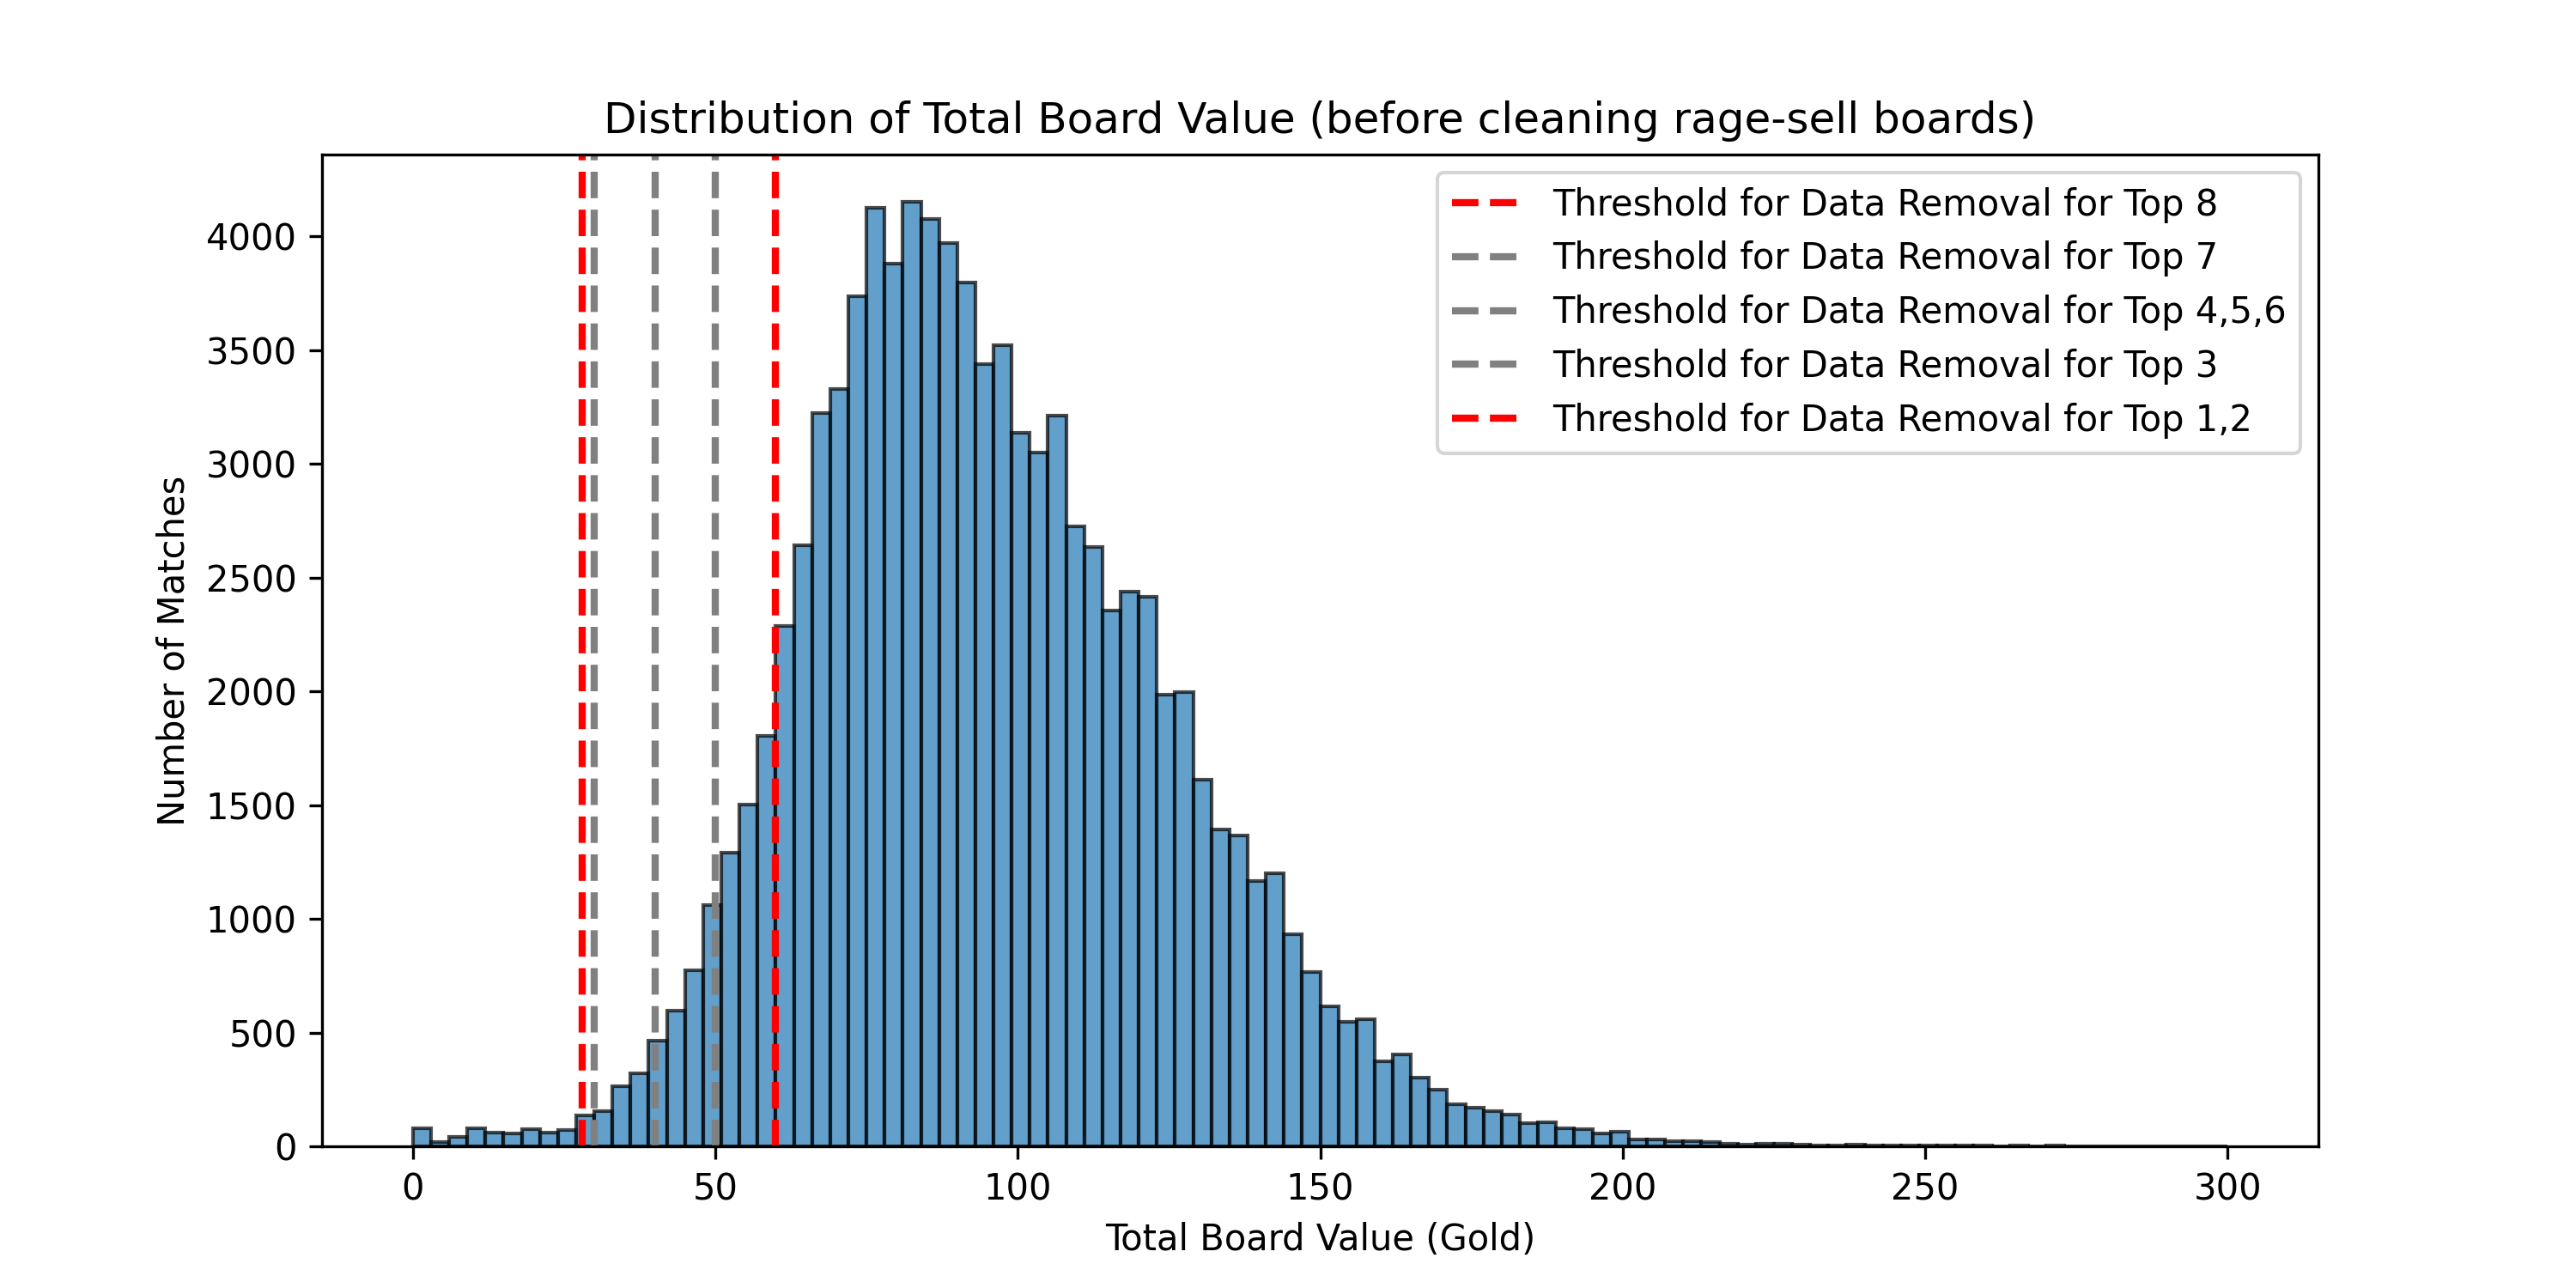
\includegraphics[width=\textwidth]{distribution_total_board_value.png}
    \caption{\label{fig:3}Representation of the data with one of our created feature : total board value}
\end{figure}

\section{Unsupervised learning}

\subsection{Objective and feature selection}
A fundamental aspect of TFT is to analyze how players construct their boards by combining units to maximize synergies. Unlike supervised learning, where the objective is to predict victory, our goal here is to explore the data using an unsupervised approach to identify the game's major archetypes, commonly referred to as "meta compositions."

To identify these compositions, we applied the K-Means clustering algorithm. Selecting the appropriate features prior to training was crucial. If we had retained "macro" variables such as player economy (gold\_left) or level (level), the algorithm would have naturally clustered players based on their in-game wealth or match pacing (grouping "rich" players together and "poor" players together). To force the algorithm to focus strictly on board identity, we isolated exclusively the categorical columns related to active synergies (e.g., syn\_TFT16\_Bruiser).

\subsection{Determining the number of clusters K via domain knowledge}
Rather than relying solely on mathematical heuristics, we determined the optimal number of clusters ($K$) using empirical testing and domain knowledge. In TFT, game balance dictates that a given patch typically features around 10 highly viable "meta" compositions, with the remainder being niche or strictly suboptimal.
Based on this premise, we iteratively tested values starting from K = 8. We observed that setting K \textgreater 10 yielded diminishing returns, as the algorithm began generating redundant sub-variations of already established compositions rather than distinct new compositions. Consequently, we validated K = 10 as the optimal parameter.

\begin{figure}[H]
    \centering
    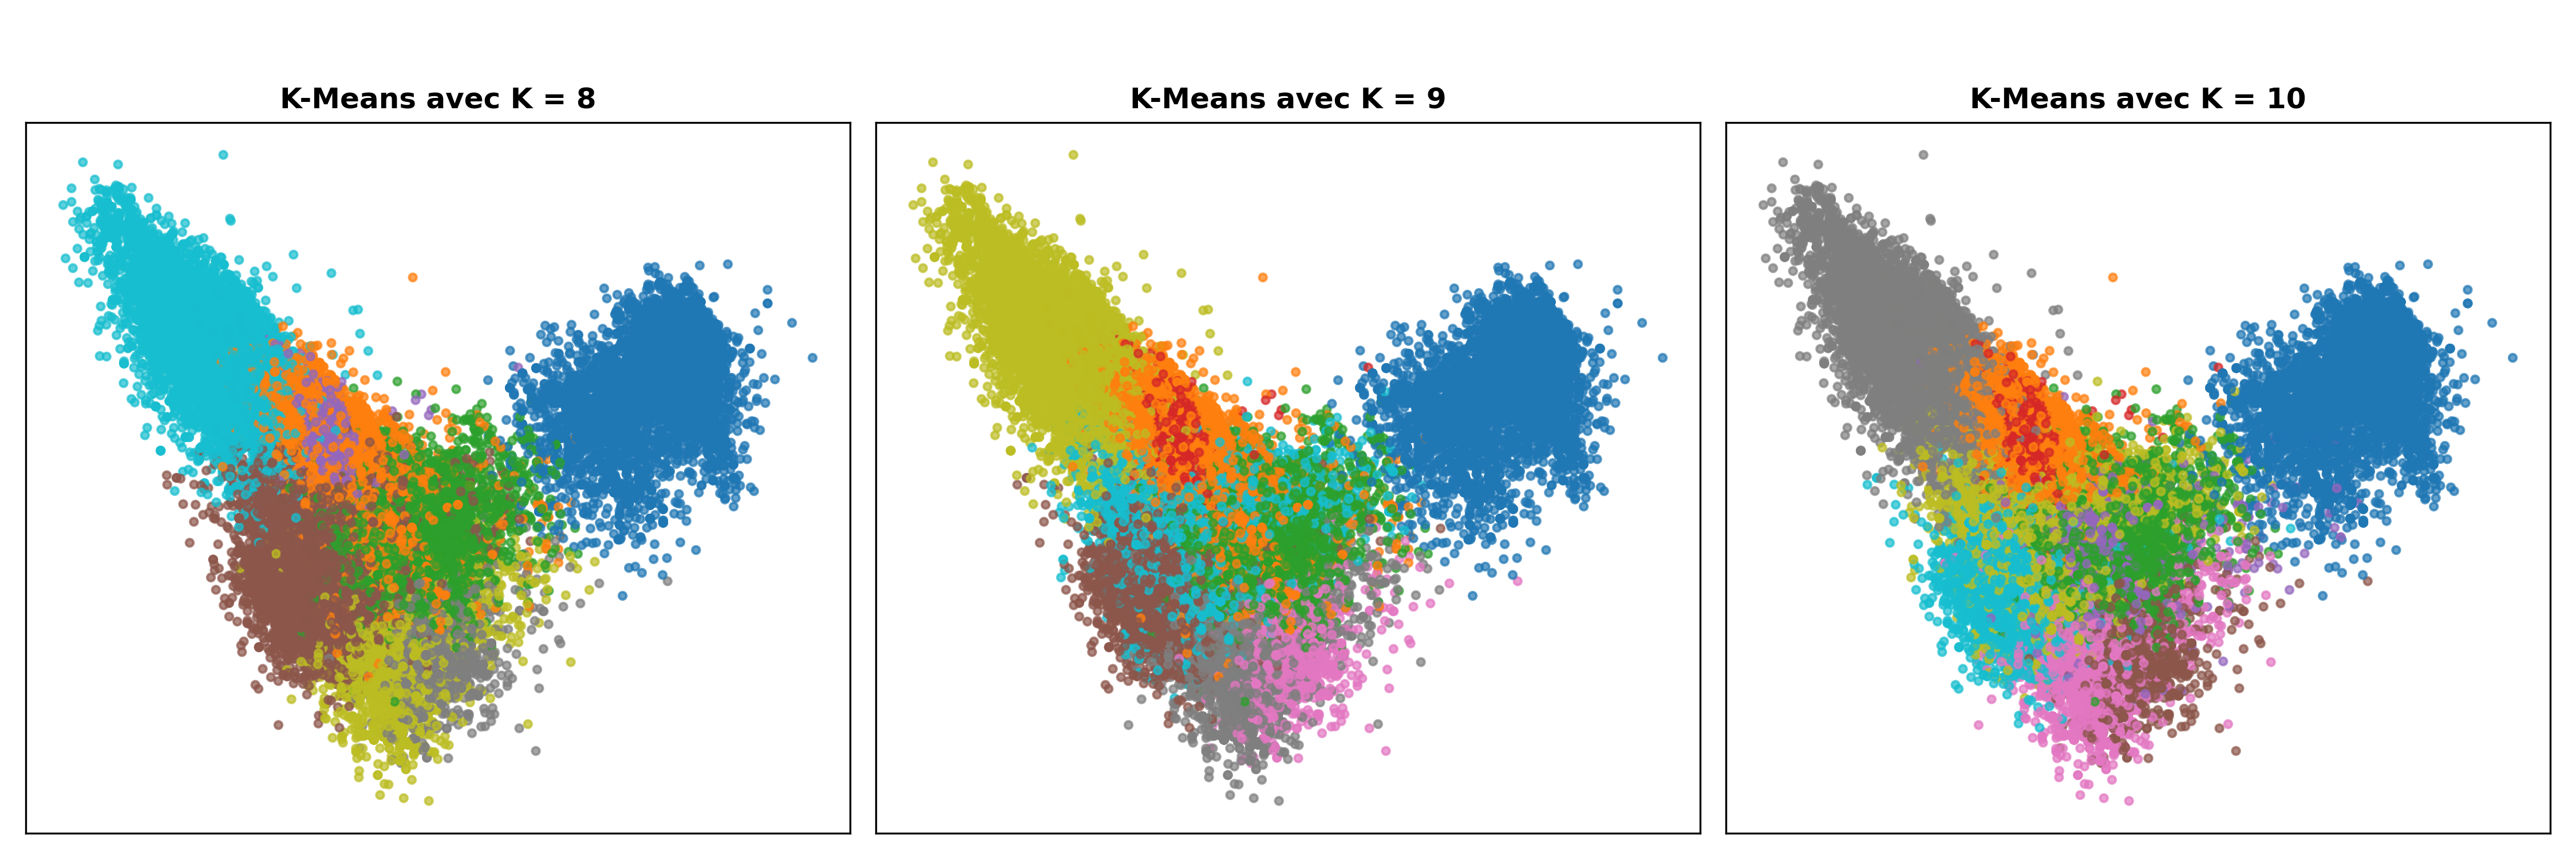
\includegraphics[width=\textwidth]{clusters_evolution.png}
    \caption{\label{fig:4}Visualisation of the K-means with different K values}
\end{figure}

\subsection{Cluster interpretability: synergies and key champions}

Upon analyzing the profiles of the 10 generated clusters, we encountered an interpretability challenge: looking solely at the average synergies was insufficient to fully grasp the identity of a composition. To accurately define an archetype, we needed to identify the specific champions activating those synergies, as these units act as the core "carries" or tanks of the board.

By mapping the most prominent synergies of each cluster to their most frequently associated champions, the true in-game compositions perfectly emerged.

\begin{figure}[H]
    \centering
    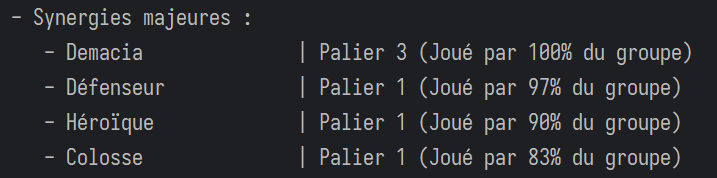
\includegraphics[width=5cm]{image_0.png}
    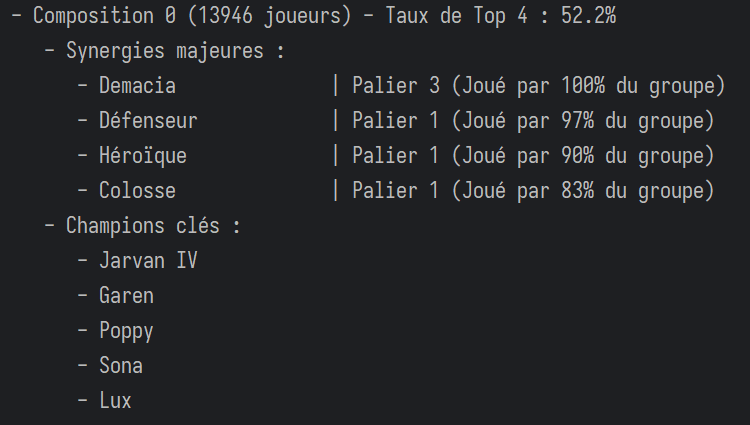
\includegraphics[width=8cm]{image_1.png}
    \caption{\label{fig:5}First attempt only with synergies, then with units}
\end{figure}

This dual analysis of synergies and units allowed us to seamlessly translate raw mathematical clusters into recognizable TFT compositions.

Example of the Ionia Yunara/Wukong composition :
\begin{figure}[H]
    \centering
    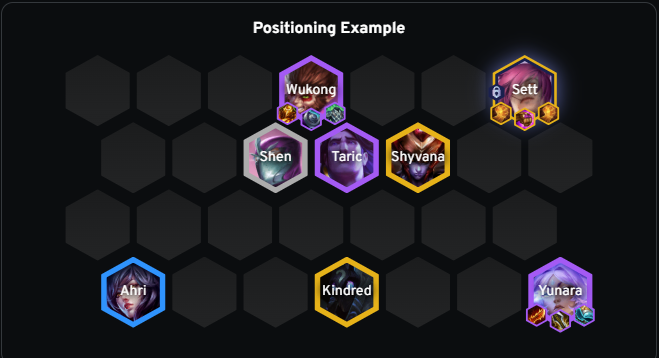
\includegraphics[width=8cm]{image_2.png}
    \caption{\label{fig:6}The TFTAcademy recommanded version of the composition}
\end{figure}

\begin{figure}[H]
    \centering
    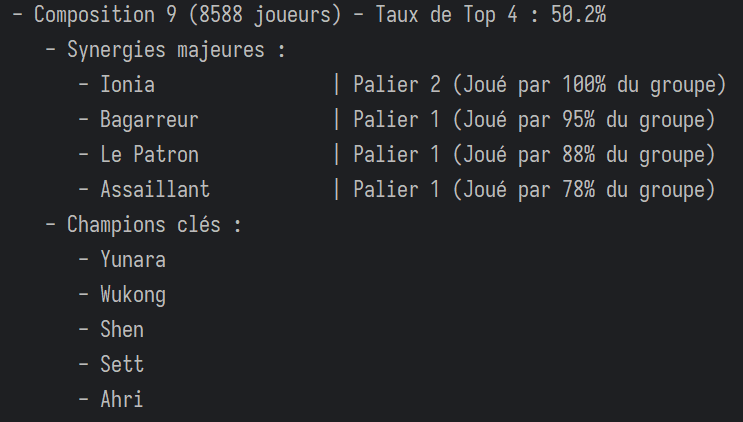
\includegraphics[width=8cm]{image_3.png}
    \caption{\label{fig:7}Results found using our K-Means algorithm}
\end{figure}


\subsection{The "rigid meta" phenomenon: why the clustering is accurate}

The algorithm successfully isolated actual in-game compositions without creating irrelevant "catch-all" groups. The high accuracy of these clusters can be attributed to the behavioral patterns of the player base, particularly at high elo.
Top-tier players constantly theory craft to find the mathematically optimal boards, aiming to maximize relevant synergies while fielding the highest-value units possible. Because every unit in an optimized composition serves a specific purpose, it is rare and often suboptimal to deviate from the established formula. Furthermore, the community heavily relies on specialized tier-list websites (such as TFTAcademy). Consequently, players naturally gravitate toward replicating these exact, pre-optimized boards, creating dense, well-defined clusters in the dataset.

\subsection{Conclusion: win rates and the cost of deviation}

We can conclude that the meta in TFT is highly rigid and quantifiable. Our K-Means model clearly demonstrated the existence of a strict meta, autonomously identifying the community's dominant compositions.
By cross-referencing these 10 clusters with their respective win rates, we obtained numerical proof that certain compositions (such as the Bilgewater-oriented board) strictly outperform others in the 16.2 patch. Furthermore, the data confirms that players who deviate too far from these optimal clusters often suffer from drastically lower win rates.


\begin{figure}[H]
    \centering
    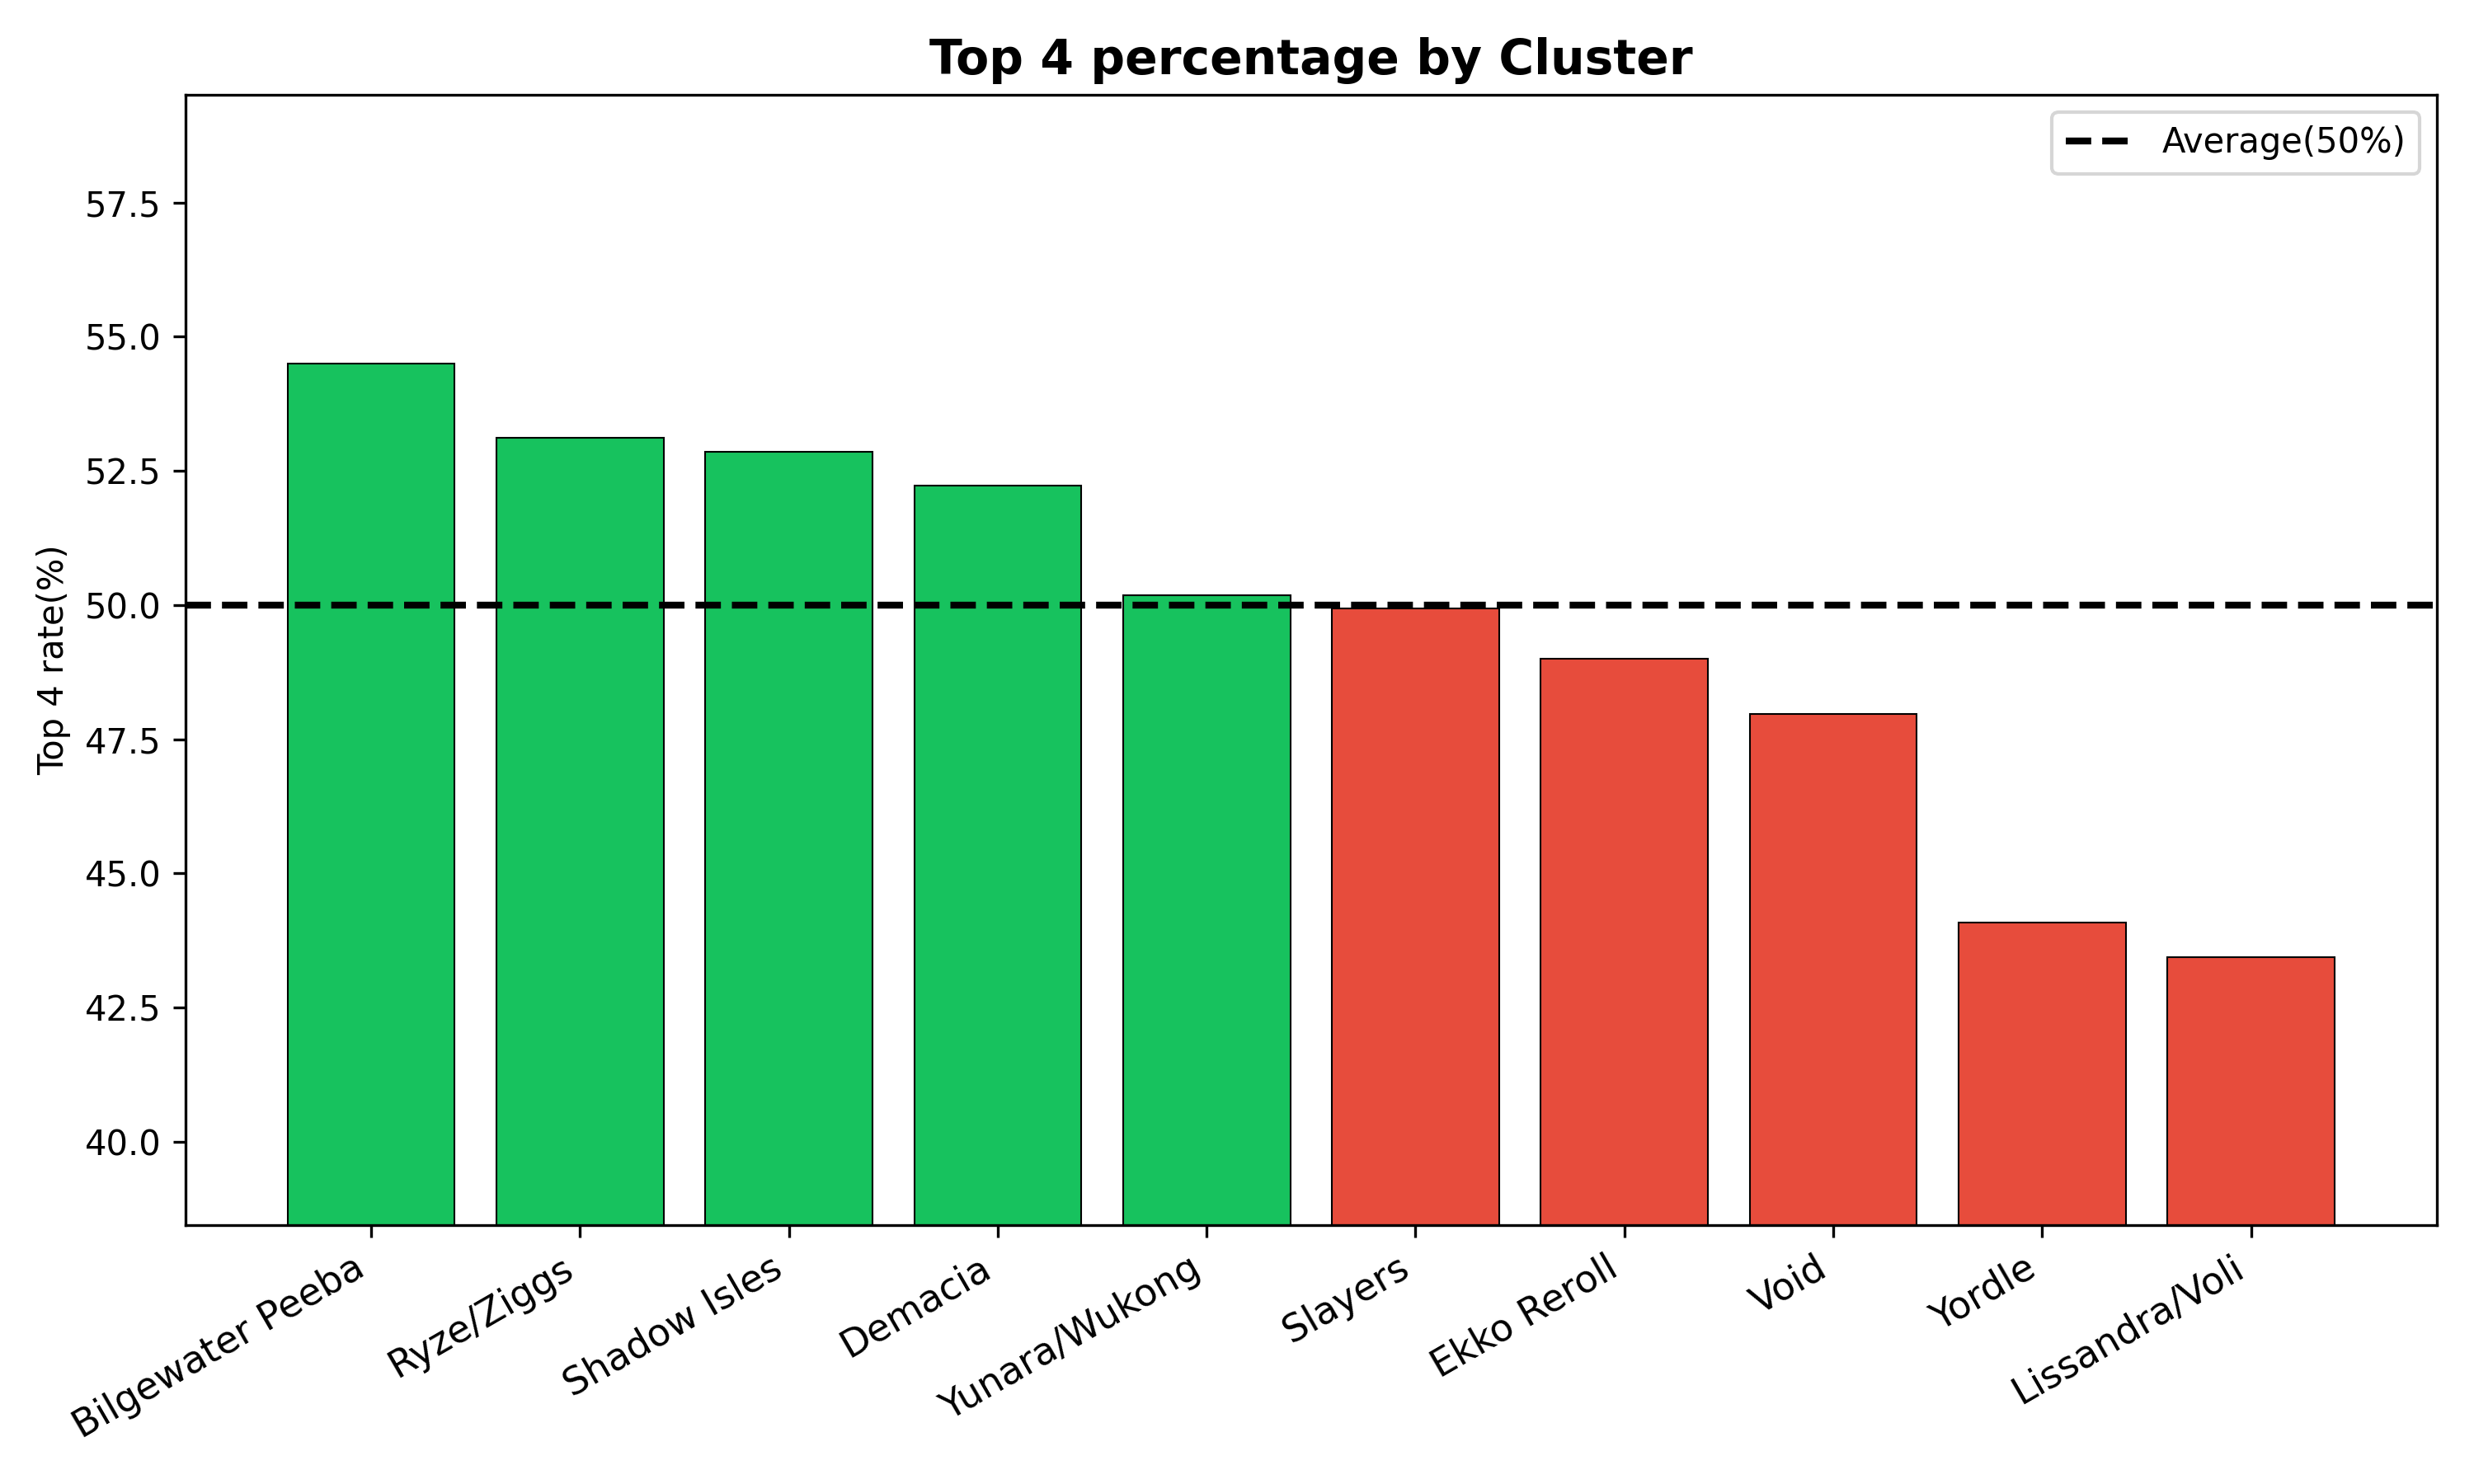
\includegraphics[width=\textwidth]{clustering_comps.png}
    \caption{\label{fig:8}The 10 most performant compositions found by the K-Means algorithm}
\end{figure}

\section{Supervised learning}

\subsection{Linear regression to find the best item on a certain unit}

\subsubsection{Intro}
In Teamfight Tactics (TFT), the final placement of a player (ranked from 1st to 8th) is influenced by a multitude of overlapping factors. To optimize gameplay, it is crucial to understand the isolated impact of a single decision, such as equipping a specific item on a specific unit. We chose linear regression for this task because it is highly effective at modeling the relationship between a dependent target variable (final placement) and multiple independent binary variables (the presence or absence of specific items on a unit).

The primary purpose of using linear regression here is to isolate the marginal effect of each item. While raw averages might be skewed by the overall strength of a composition, the regression algorithm mathematically controls for the environment, assigning a specific weight to the item itself. This allows us to answer a precise question: how much does equipping this specific item on this specific unit affect my final rank?

\subsubsection{Explaining delta}
In our model, the regression coefficient ($\beta$) assigned to an item-champion combination is referred to as the Delta. In the context of TFT statistics, the Delta represents the expected change in a player's final placement when that specific choice is made. Because the ultimate goal in TFT is to achieve a lower placement number (e.g., 1st place is better than 8th place), the interpretation of the Delta is inverted compared to standard performance metrics: A negative Delta (e.g., -0.45) is highly beneficial. It means the item mathematically reduces the player's final placement score by 0.45 positions, pushing them closer to 1st place. A positive Delta (e.g., +0.30) is detrimental, indicating that the item pushes the player further down the standings toward 8th place


\subsubsection{Context and model variability}
As part of our supervised learning analysis, we utilized linear regression to determine the optimal itemization for specific units, using the champion Ziggs as our primary case study. The results demonstrated that the model's predictive accuracy is heavily dependent on the selected unit. While the regression yielded excellent precision in identifying the "Best-in-Slot" (BiS) items for champions like Ziggs, the performance fluctuated for other units. This variance is expected, as itemization in Teamfight Tactics is a highly contextual decision influenced by numerous in-game factors (e.g., augments, item economy, enemy compositions and more...). Nevertheless, the model consistently demonstrated strong accuracy in isolating the top-performing items for a given carry.


\begin{figure}[H]
    \centering
    
\includegraphics[width=\textwidth]{bis_item_ziggs.png}
    \caption{\label{fig:9}Best items on the Character 'Ziggs' obtained using linear regression}
\end{figure}

\subsubsection{Methodology and external validation}
To validate our findings, we compared the impact scores (Deltas) extracted from our linear regression coefficients with empirical data provided by specialized tracking platforms (such as \href{tactics.tools}{Tactics.Tools}). While these websites calculate raw statistical deltas directly by averaging match history occurrences, our approach derives the delta mathematically through regression, isolating the specific impact of the item. The strong alignment between our model's mathematical predictions and these external empirical statistics confirms the reliability of our approach.

\begin{figure}[H]
    \centering
    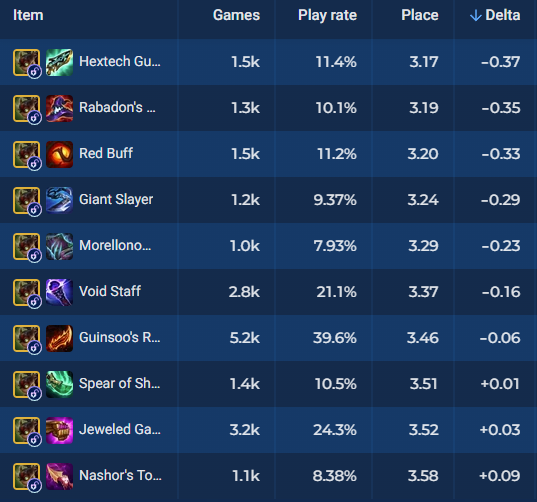
\includegraphics[width=8cm]{image_4.png}
    \caption{\label{fig:10}Items with the best delta on Ziggs found on the Data Explorer of tactics.tools (considering a larger playerbase)}
\end{figure}

\subsubsection{Data sparsity and implicit survivor bias}
A notable observation from our Linear Regression results is the near absence of items with highly positive deltas (which indicates poor performance). This phenomenon is a direct consequence of the dataset's nature and our preprocessing.

During the data cleaning phase, features representing specific champion-item combinations were dropped if their non-zero occurrence rate fell below a strict threshold (e.g., \textless 0.003). Because our dataset comprises top-tier players, they naturally avoid equipping objectively detrimental items on a unit (for instance, equipping tank or attack damage items on Ziggs, who is strictly an ability power carry).

Consequently, these mathematically suboptimal items rarely appear in the dataset, leading to their removal during preprocessing. Therefore, the sheer lack of occurrences for these items acts as an implicit indicator of their poor performance. The regression model primarily evaluates items that are already considered viable by high-elo players, which logically explains why the resulting deltas are predominantly negative (beneficial) or neutral.


\subsection{Predicting match outcomes}

\subsubsection{Baseline comparison: the failure of Naive Bayes}
To predict whether a player will achieve a victory (Top 4 finish), we initially evaluated a Naive Bayes classifier as our baseline model. However, 5-fold cross-validation yielded an average accuracy of only 68.23\% (with a narrow standard deviation of $\pm$ 0.47\%).

The reason for this underperformance lies in the algorithm's fundamental mathematical assumption: Naive Bayes assumes that all features are strictly independent. In a game like Teamfight Tactics, this assumption completely collapses. The strength of a unit is directly dependent on the synergies activated around it and the items equipped. To capture these highly complex, non-linear relationships, we transitioned to a tree-based ensemble method: the Random Forest Classifier.

\begin{figure}[H]
    \centering
    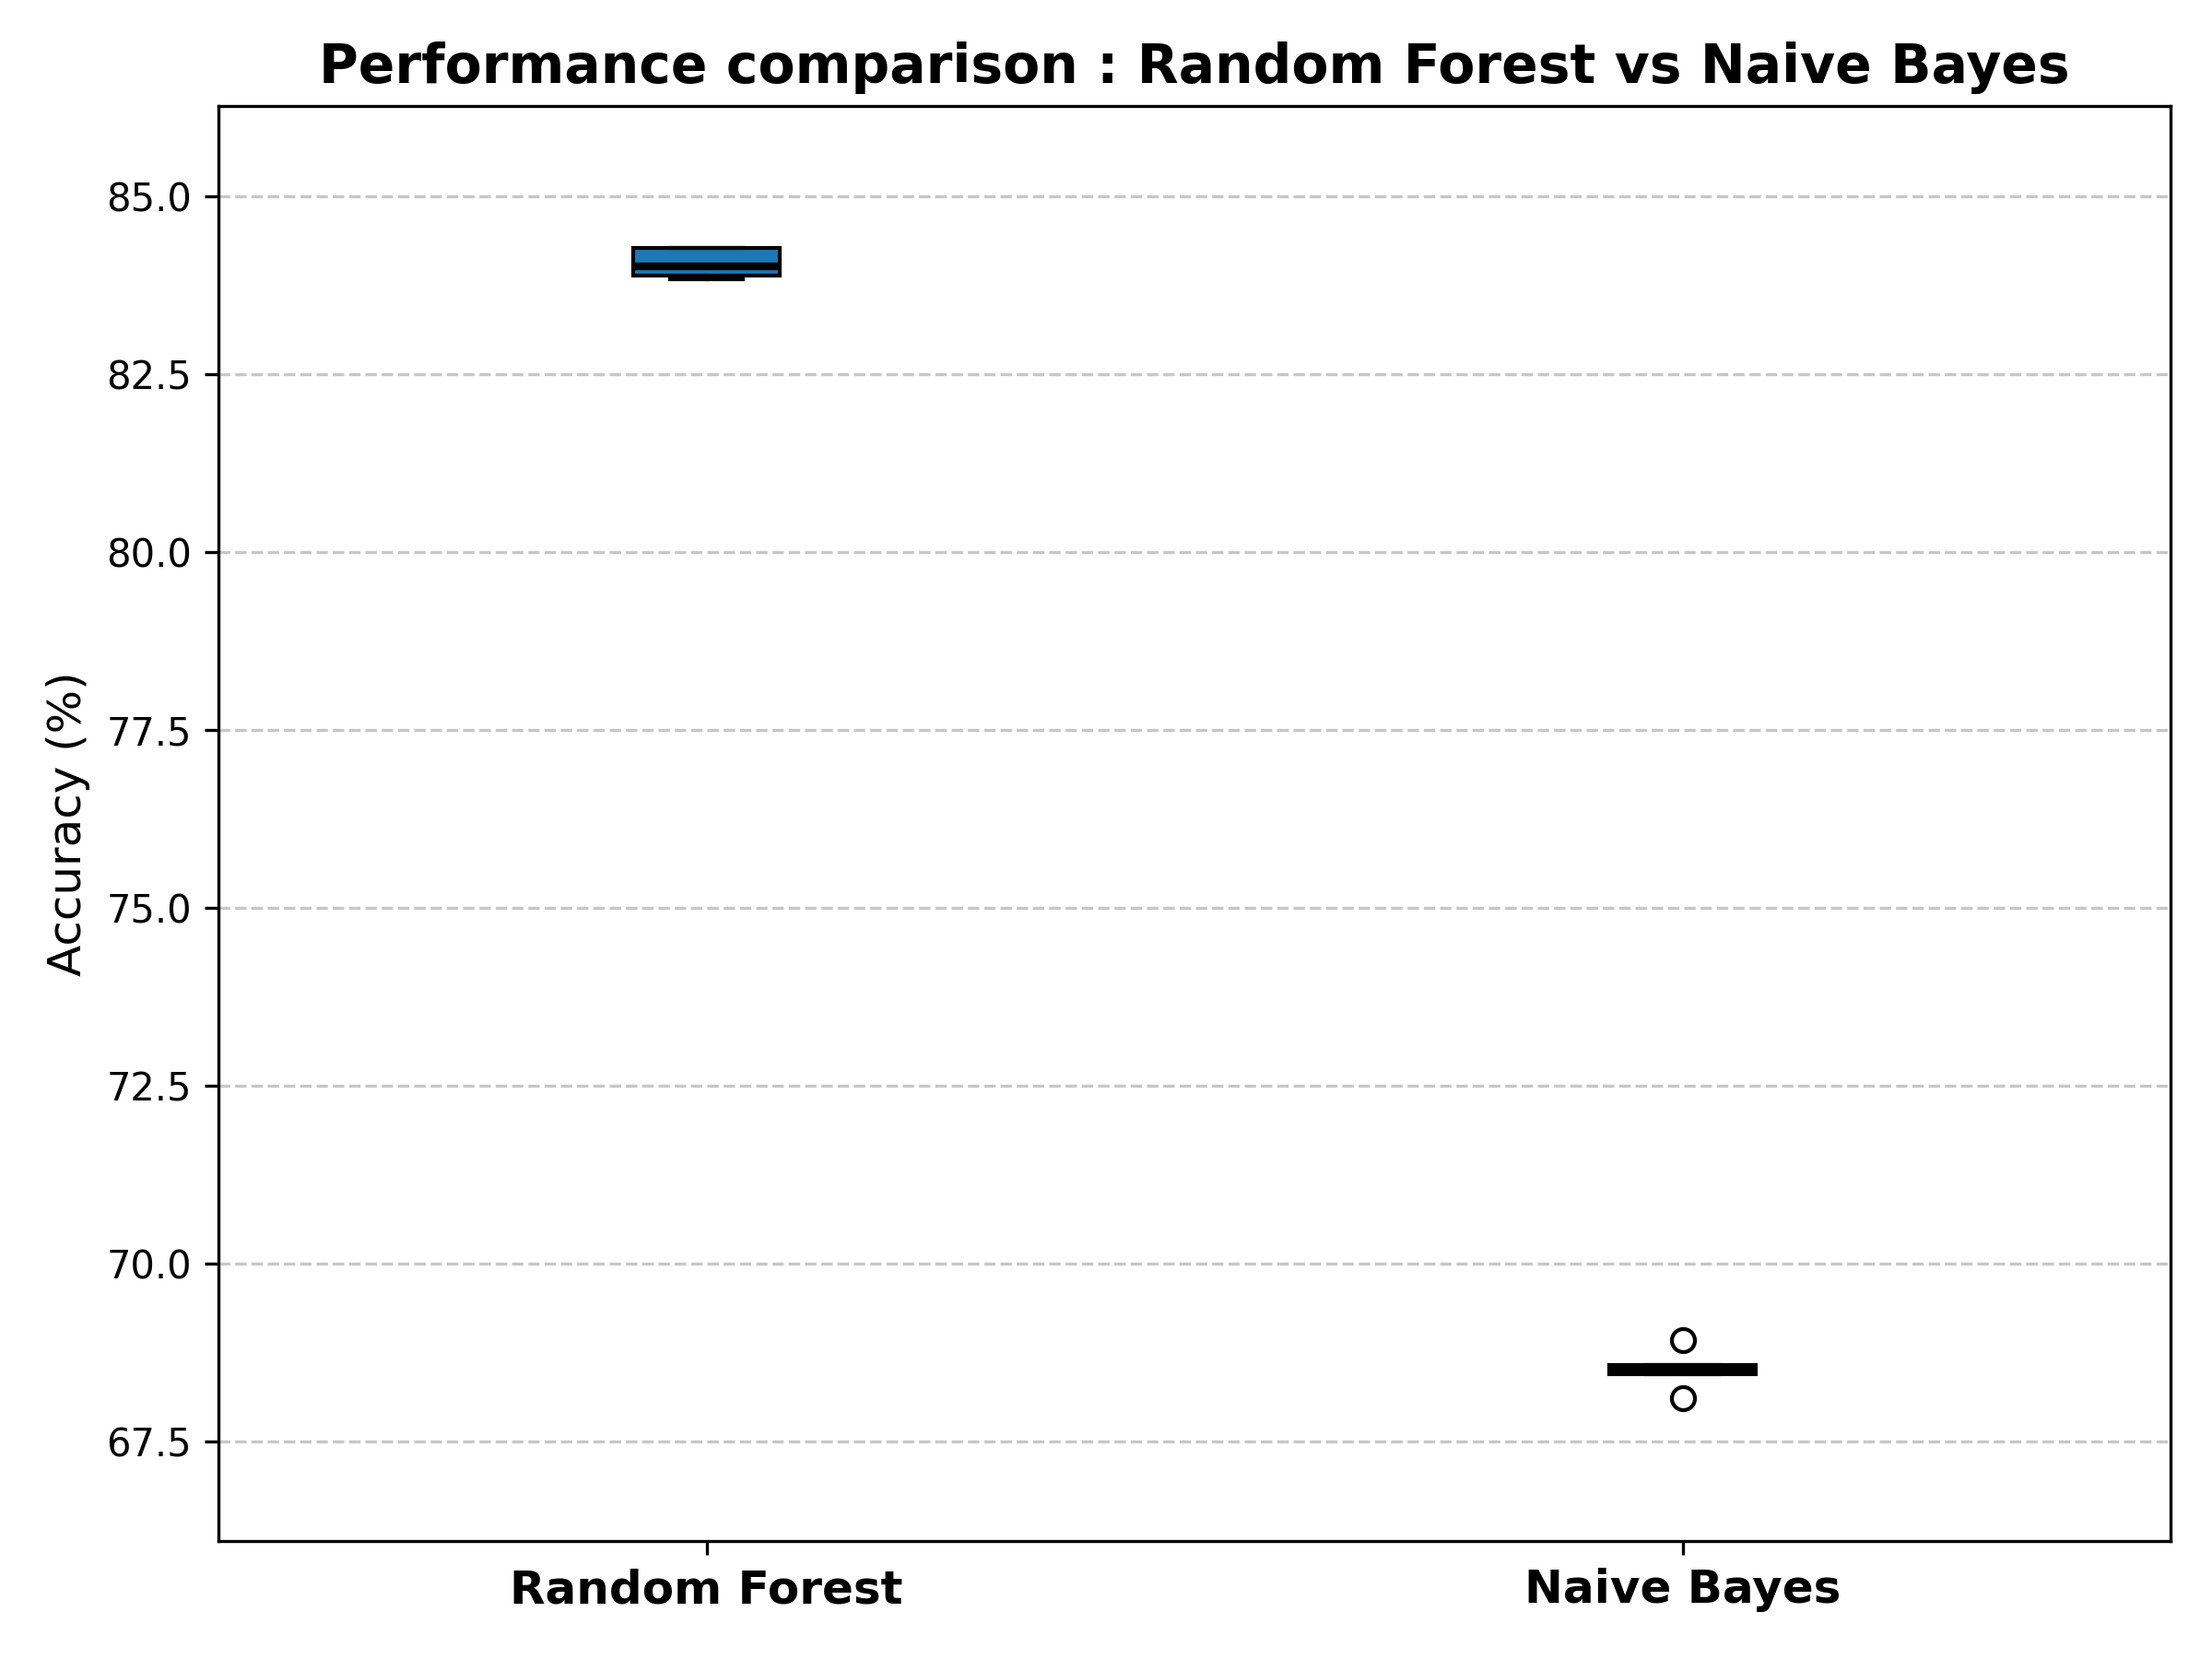
\includegraphics[width=\textwidth]{nb_vs_rf.png}
    \caption{\label{fig:11}The boxplot of Naives Bayes versus Random Forest GroupKFold predictions }
\end{figure}

\subsubsection{Evaluation strategy: preventing data leakage}
To train and evaluate the Random Forest, we compared two different data splitting methodologies:

Classic train/test split: This standard approach yielded a global accuracy of 83.53\%.

Group shuffle split (by Match ID): Because TFT is played in lobbies of 8 players where the economy and unit pools are shared, players from the same match are inherently correlated. Splitting players from the same lobby across both the training and testing sets introduces data leakage. By grouping the split by match\_id, we ensured the model was evaluated on entirely unseen lobbies. Under this stricter and more realistic evaluation, the model achieved an improved global accuracy of 83.92\%.

\subsubsection{Model performance and stability}
Using the group shuffle split, the Random Forest demonstrated excellent predictive capabilities. The confusion matrix on the test set is detailed below:

\begin{figure}[H]
    \centering
    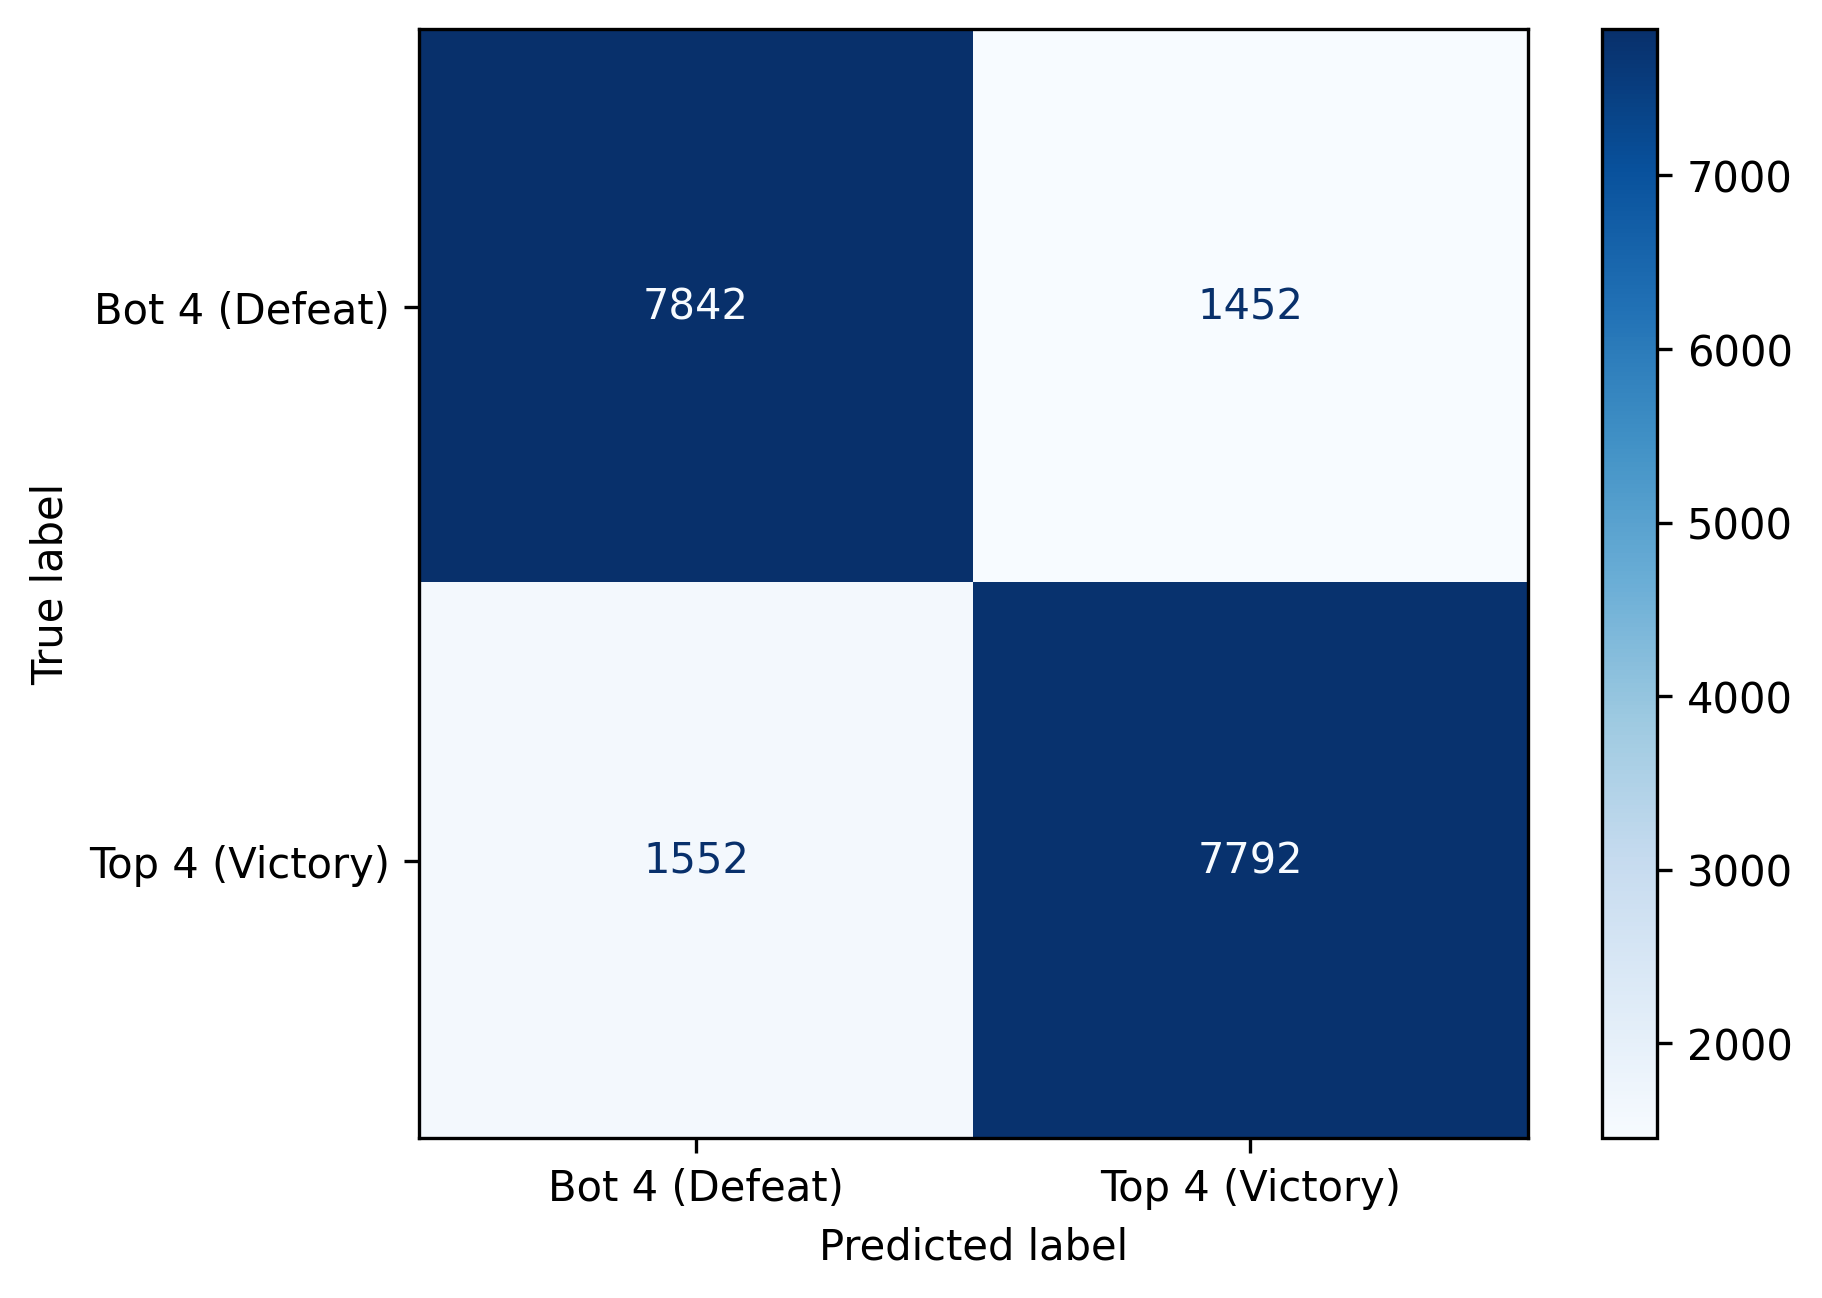
\includegraphics[width=10cm]{confusion_matrix.png}
    \caption{\label{fig:12}The confusion matrix}
\end{figure}

The classification report shows a highly balanced performance, with both Precision, Recall, and the F1-score stabilizing at 0.84 across both classes. Furthermore, extensive cross-validation confirmed that these scores are highly stable, proving that the model is robust and does not suffer from overfitting.

\begin{figure}[H]
    \centering
    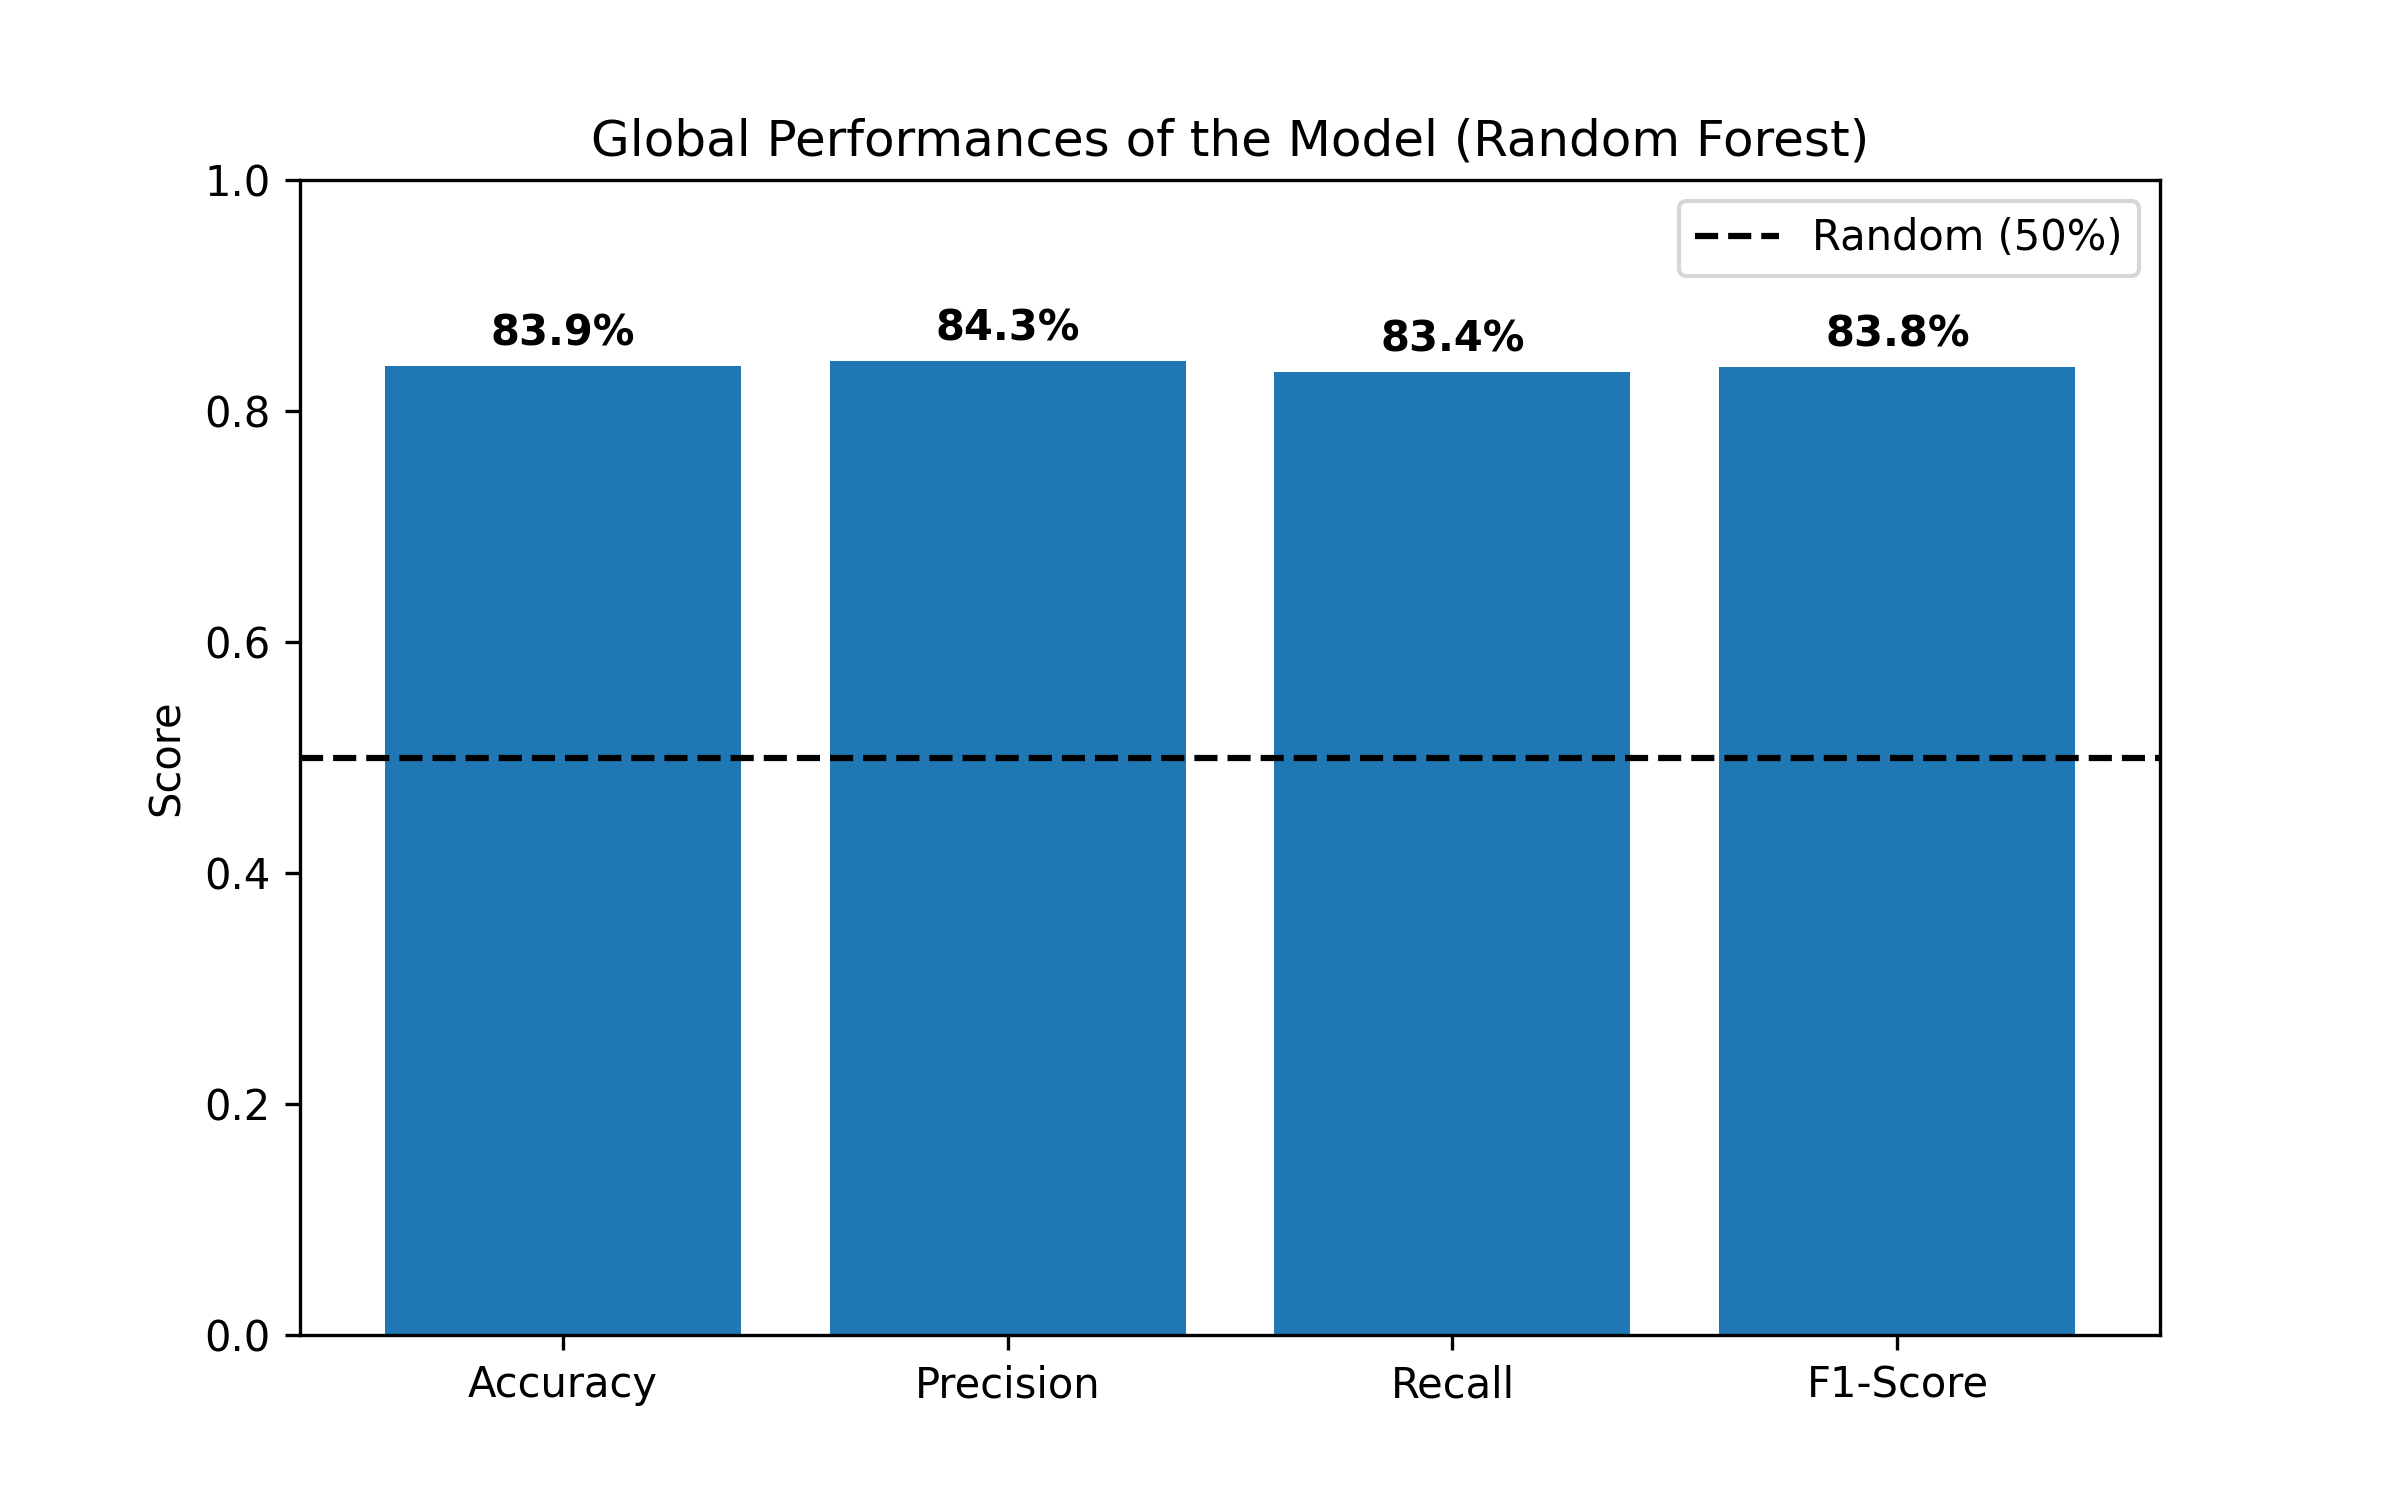
\includegraphics[width=15cm]{accuracy_precision_recall_f1.png}
    \caption{\label{fig:13}Accuracy, Precision, Recall, and F1 scores}
\end{figure}

To further validate the performance of our Random Forest, we plotted the ROC curve and calculated the AUC. The AUC reaches 0.92, which is an excellent score (a completely random model would have an AUC of 0.50).

This result demonstrates that our model does not merely achieve good overall accuracy, but also possesses an excellent discrimination capacity: it can highly reliably separate compositions destined for a Top 4 finish from those destined for a Bot 4, with a minimum of false positives. This strongly validates the robustness of the features extracted during our analysis.

\begin{figure}[H]
    \centering
    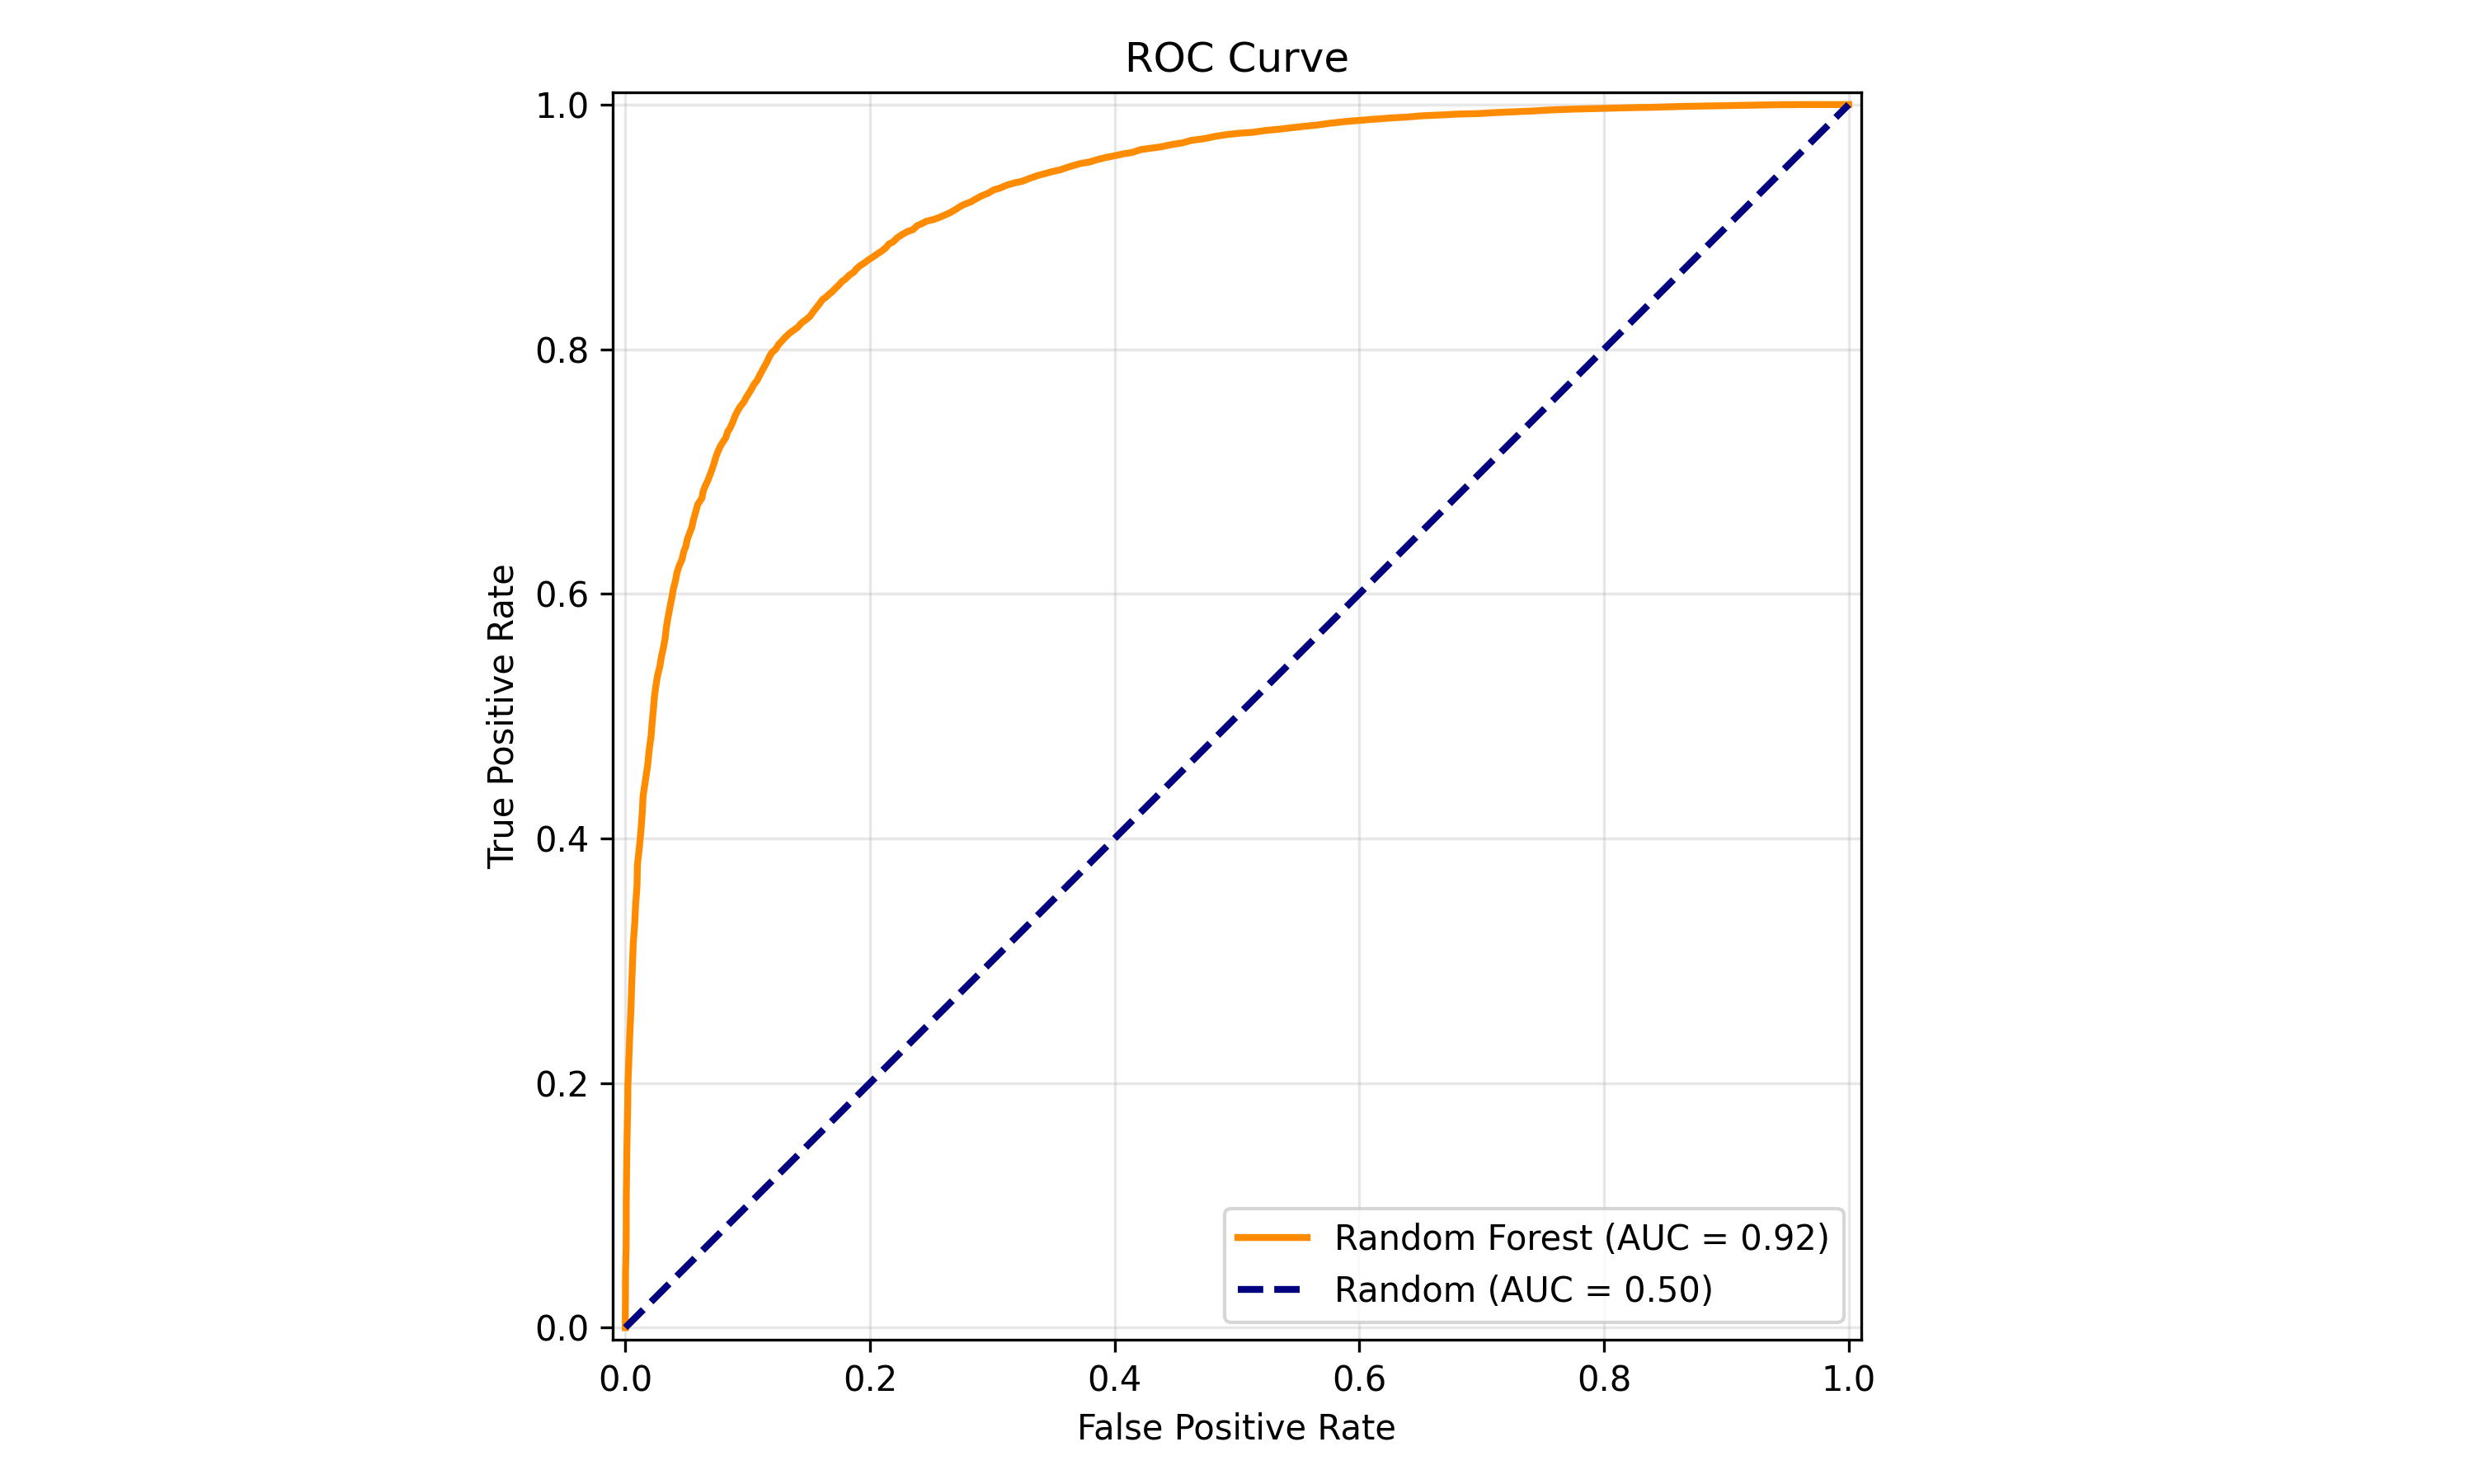
\includegraphics[width=15cm]{roc_curve.png}
    \caption{\label{fig:14}ROC Curve}
\end{figure}

\subsubsection{Hyperparameter optimization}
To push the model to its maximum potential, we performed Hyperparameter tuning using GridSearchCV. The optimization process concluded with a peak cross-validated accuracy of 84.13\%.

The optimal hyperparameters identified by the grid search were:

n\_estimators: 200 (Creating a dense forest of 200 decision trees).

max\_depth: None (Allowing the nodes to expand until all leaves are pure, capturing the deepest edge-case combinations of the game).

min\_samples\_leaf: 1 (Allowing fine-grained splits).

\subsubsection{Feature importance analysis: macro over micro} 
One of the most valuable outputs of a Random Forest is its ability to rank the variables that most heavily influence its decisions. However, before analyzing the results, it is important to highlight a specific feature engineering choice we made regarding the nature of the game.

Because TFT is a zero-sum game played in closed lobbies of 8 players, a player's performance is strictly relative to their specific opponents. An absolute board value of 50 gold might be overwhelming in a low-rolling lobby, but entirely insufficient in a high-rolling one. To capture this lobby dependency and measure a player's strength compared to their direct opponents, we engineered relative variables, namely ratio\_valeur\_plateau (board value relative to the lobby) and ratio\_level (Level relative to the lobby).

Analyzing the feature importances revealed a clear hierarchy in what the model uses to determine a victory:

\subsubsection{The dominance of macro fundamentals}
The top of the hierarchy is entirely monopolized by "macro" variables:

\begin{figure}[H]
    \centering
    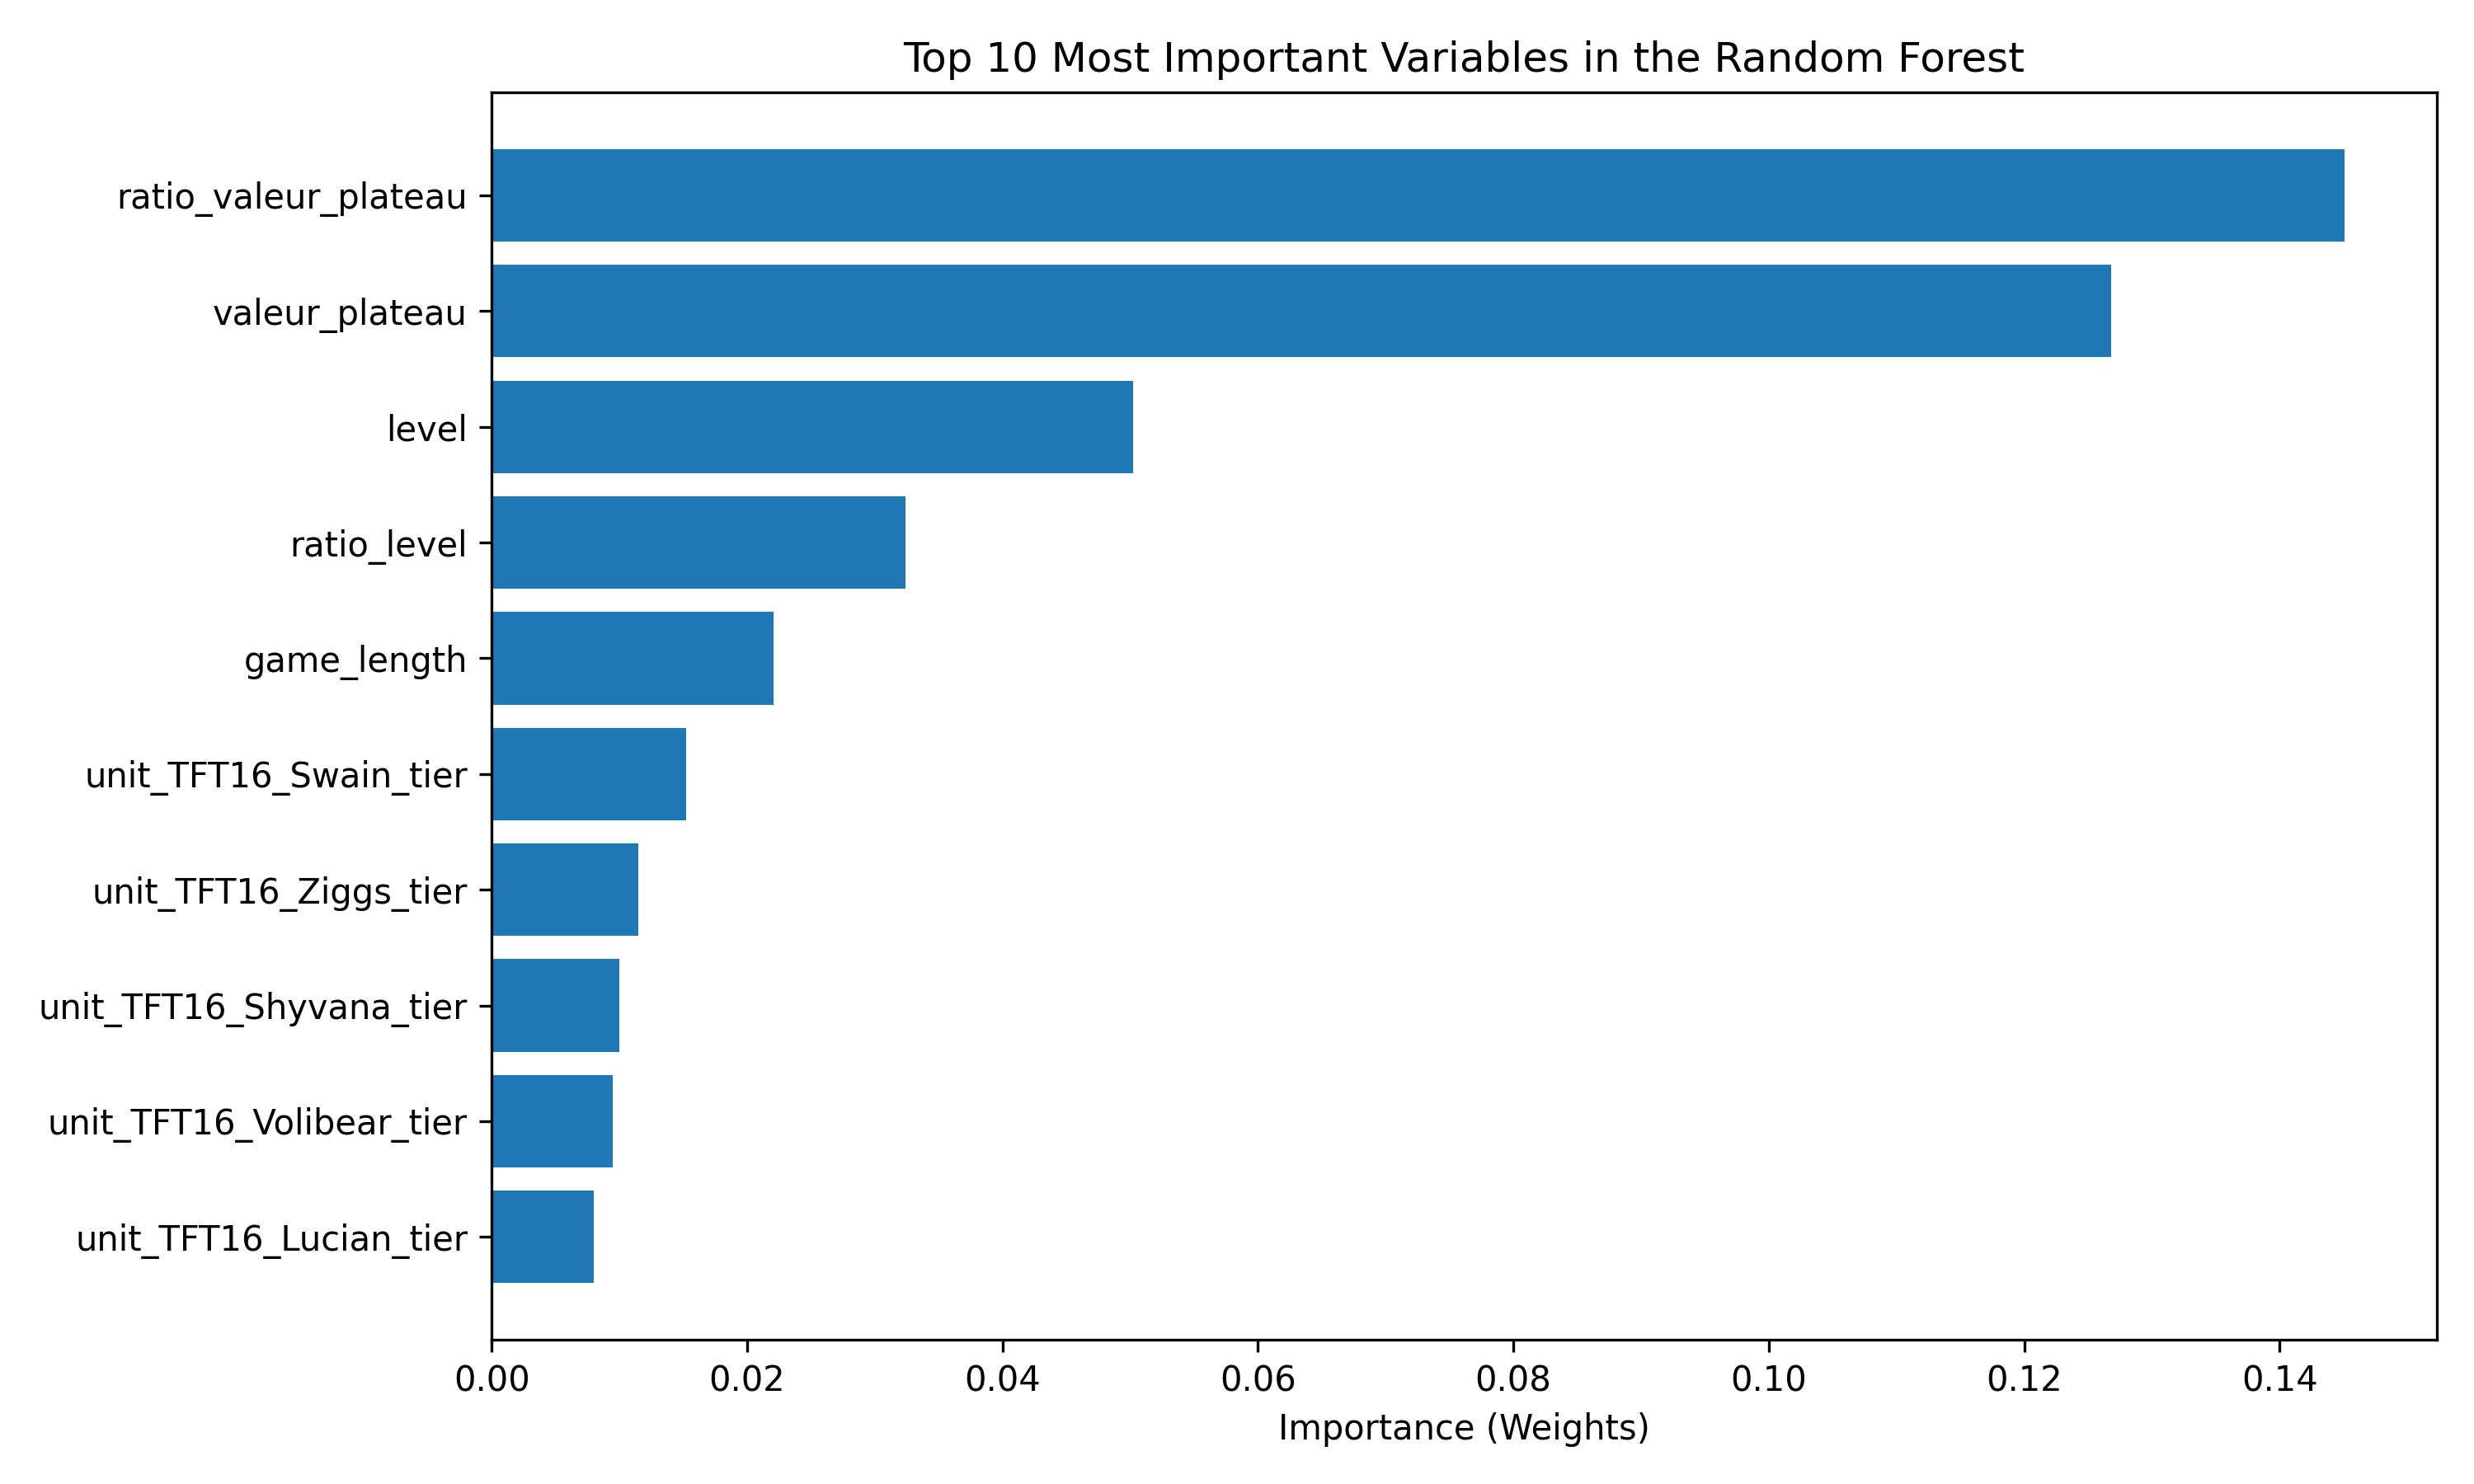
\includegraphics[width=\textwidth]{most_important_variables.png}
    \caption{\label{fig:15}Most impactful variables in the Random Forest}
\end{figure}

The fact that the relative ratios significantly outperform the absolute values proves our initial hypothesis: success in TFT is primarily about outpacing the specific lobby you are in. These metrics highlight that raw board value (the cost and star level of the units) and experience (level) are the strongest measurable drivers of victory.

\subsubsection{A critical nuance: the missing data of augments}
While one might be tempted to look at these percentages and conclude that raw board value will always outperform a perfectly synergized but cheaper composition, making such a definitive statement would be incorrect.

Our model currently lacks a fundamental dimension of modern TFT gameplay: Augments. Augments provide massive, game-altering power spikes that can easily allow a cheaper, highly synergized board to defeat a more expensive, disjointed one. Unfortunately, Riot Games removed augment information from their public API a few years ago, making it impossible to scrape and integrate into our dataset.

Consequently, while board value and level are the absolute dominant predictive factors available in our data, we must acknowledge that they are part of a broader, partially unquantifiable ecosystem where hidden variables like augments play an equally decisive role in the reality of the game.

\subsubsection{The micro factors and meta validation}
When looking past the macro variables, the highest-ranking specific champion in the dataset is Ziggs, holding a 1.22\% influence, closely followed by Swain (1.17\%) and Shyvana (0.98\%).

\subsubsection{The expected dominance of high-cost units and the Ziggs meta}
From a game design perspective, it is statistically expected that high-cost champions rank highest among individual units, as they possess inherently superior base stats and high-impact abilities. The prominence of Ziggs is a perfect example of this, aligning flawlessly with empirical domain knowledge. During patch 16.2 (the environment from which this data was extracted), the community widely recognized the Ziggs/Ryze composition as the absolute strongest board in the meta. The Random Forest independently learned this meta-dynamic simply by correlating the presence of Ziggs with a disproportionately high probability of a Top 4 finish.

\subsubsection{The Swain and Shyvana synergy}
The presence of Swain and Shyvana just behind Ziggs provides another fascinating insight into how the algorithm understands the game. Their high ranking is not a coincidence; rather, it reflects a highly optimized late-game duo. Both units share the Juggernaut trait, meaning fielding them together immediately activates the 2-Juggernaut synergy, adding immense value to almost any late-game board.

Furthermore, the model accurately captures their exceptional dual role as both frontline tanks and utility engines:

Swain: His ability allows him to stun a large portion of the enemy board, providing massive crowd control that can single-handedly swing the outcome of late-game team fights.

Shyvana: She is a highly efficient unit that does not strictly require item investments to absorb hits or deal respectable damage. Additionally, she possesses a unique passive ability that grants bonus tankiness to the entire team.

Ultimately, the Random Forest successfully identified that fielding this specific duo grants a massive tactical advantage. Their combined crowd control, trait synergy, and team-wide survivability make them quintessential components of a winning board, perfectly explaining why the algorithm assigned them such a high predictive weight together.

\end{document}